\documentclass{beamer}

\usepackage{color} % Package to include colors for syntax highlighting
\usepackage{graphicx}  % Package to include images
\usepackage{hyperref}  % Hyperlinks
\usepackage{tikz}

\setbeamertemplate{navigation symbols}{}  % Remove navigation symbols
\usecolortheme[light]{solarized}

\title{Mid module feedback}
\date{}


\begin{document}

\frame{
    \titlepage
}

\frame{
    \begin{center}
        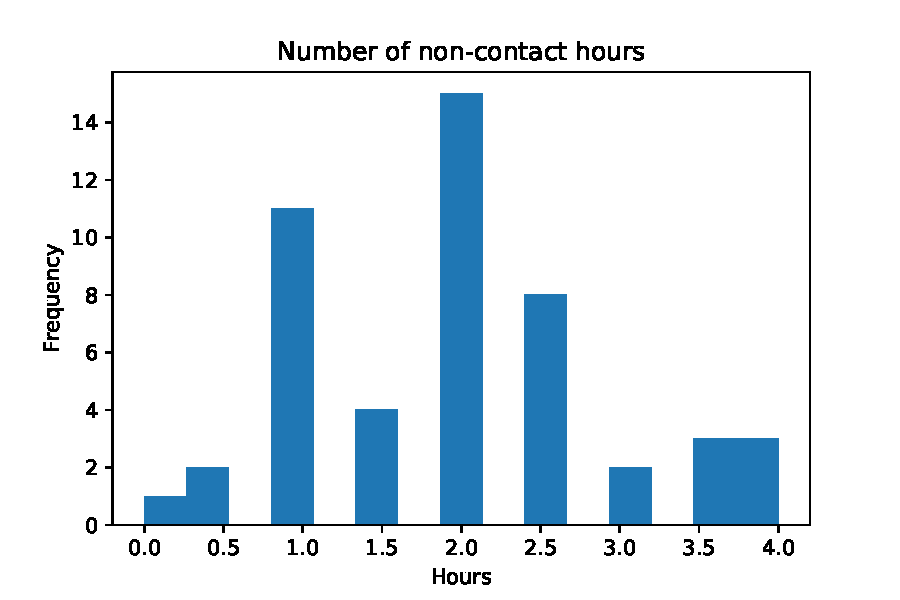
\includegraphics[width=.8\textwidth]{plot.pdf}
    \end{center}
}

\frame{
    \Large
    \begin{quote}
        Worksheets: good.
    \end{quote}
}

\frame{
    \Large
    \begin{quote}
        Class meetings: good.
    \end{quote}
}

\frame{
    \Large
    \begin{quote}
        Extra resources: good.
    \end{quote}
}

\frame{
    \Large
    \begin{quote}
        Videos: good.
    \end{quote}
}

\frame{
    \Large
    \begin{quote}
        Lab tutors: good.
    \end{quote}
}

\frame{
    \Large
    \begin{quote}
        List of topics: good.
    \end{quote}
}

\frame{
    \Large
    \begin{quote}
        Vince: good.
    \end{quote}
}


% Bad

\frame{
    \Large
    More explanation of coursework please.
}

\frame{
    \Large
    \begin{quote}
        ``Lab work to be more worked examples, not Q and A.''
    \end{quote}
}

\frame{
    \Large
    \begin{quote}
        ``Labs are too close to the lecture times.''
    \end{quote}
}


\frame{
    \Large
    \begin{quote}
        ``Getting carried away on a particular example, going really quickly
        makes it hard to copy or understand code.''
    \end{quote}
}

\frame{
    \Large
    \begin{quote}
        ``Upload documents from lectures pls.''
    \end{quote}
    \begin{quote}
        ``The code you write in lecture could possibly be made available on
        learning central.''
    \end{quote}
}

\frame{
    \Large
    \begin{quote}
        ``People are shy so the silence until someone speaks can sometimes be
        unhelpful''
    \end{quote}
}

\frame{
    \Large
    \begin{quote}
        ``Lecturer can come across as condescending and makes me feel
        discouraged to participate''
    \end{quote}

    \begin{quote}
        ``I feel like I can't ask for help because you're intimidating and I'm
        stupid.''
    \end{quote}
    \pause
    \begin{quote}
        ``Vince is very helpful''
    \end{quote}
}


\frame{
    \Large
    \begin{quote}
        ``When someone walks in late please ignore them.''
    \end{quote}
}

\frame{
    \Large
    \begin{quote}
        ``Answers to the exercises after certain amount of time.''
    \end{quote}
}

\frame{
    \Large
    \begin{quote}
        ``More examples.''
    \end{quote}
}

\frame{
    \Large
    \begin{quote}
        ``Lectures seem less useful that other modules with resort to learning
        the work but that seems by design with all the info easily available in
        youtube videos..''
    \end{quote}
}

\frame{
    \Large
    \begin{quote}
        ``Friday lectures sometimes feel like they're just repeating what was
        said on Monday.''
    \end{quote}
}

\frame{
    \Large
    \begin{quote}
        ``We don't go through the theory in the lectures.''
    \end{quote}
}

\frame{
    \Large
    \begin{quote}
        ``Sometimes tutors are unable to see where my code is wrong.''
    \end{quote}
}

\frame{
    \Large
    \begin{quote}
        ``Lack of homework means that incentive to work outside of lectures is
        hard to find.''
    \end{quote}
}

\frame{
    \Large
    \begin{quote}
    ``iOS app drains battery life.''
    \end{quote}
}

\frame{
    \Large
    \begin{quote}
    ``Nice scarf.''
    \end{quote}
}

\end{document}
